\chapter{Results}\label{ch:Results}

The dataset consists of two parts, the indexed genomes from which the Colored De Bruijn Graph is generated, and the reads which will be pseudoaligned against this index.
Firstly, the colored DBG was built using Themisto with a dataset consisting of three collections of genomes~\cite{ecoli_genomes_1, ecoli_genomes_2, ecoli_genomes_3}, which were compiled into a single collection~\cite{genomes_compilation} and is freely available on Zenodo\footnote{\url{https://zenodo.org/record/6695372#.ZFqc1c5BwQ9}}.
$k$ was chosen to be 31, as this was also the value used in previous studies of this kind~\cite{Harri, SBWT}.
This results in a DBG with $363,283,293$ vertices, $4,158,243$ dense color sets and $3,422,440$ sparse color sets, with $10,180$ total colors.

Next, the reads dataset consists of sequenced neonatal gut samples~\cite{ecoli_genomes_3} and can be found freely on the European Nucleotide Archive\footnote{\url{https://www.ebi.ac.uk/ena/browser/view/PRJEB32631}}.
The latter dataset is Terabytes large, so a subset of it was used for the feasibility of running benchmarks on the devices available.
The names of the files in this subset may be found in Appendix~\ref{app:file_names}.
The resulting size of this subset is 14.784 GB when each file is zipped individually, and 50.265 GB when unzipped.
In terms of its contents, the subset contains $226,973,768$ sequences, $22,477,526,692$ characters and $15,668,313,652$ $k$-mers.

In terms of hardware, two nodes from two different supercomputers were used, both of which are owned by \textit{CSC - IT Center for Science} located in Finland.
The first machine is called Mahti\footnote{\url{https://docs.csc.fi/computing/systems-mahti/}}, which has NVIDIA GPUs and thus the code is transpiled from HIP to CUDA code.
LUMI\footnote{\url{https://www.lumi-supercomputer.eu/lumis-full-system-architecture-revealed/}} is the second machine, which has AMD GPUs and therefore, in this case, the code is transpiled to ROCm\texttrademark.
On both machines, 400GB of memory was reserved to be used, however not all of this is used since, in terms of memory, the GPU memory is usually not sufficient to keep up with this abundance of main memory.
The actual memory used will be discussed later in this section.
For the important distinctions between the two machines and the hardware specifications with which the code was run, the reader is invited to look at Table~\ref{tab:Specifications}.
The number of threads is double that of the core counts due to simultaneous multi-threading\footnote{\url{https://www.ibm.com/docs/en/aix/7.2?topic=concepts-simultaneous-multithreading}}, on both machines.

\begin{table}[]
\centering
\caption{Comparing specification and baseline benchmarks of the two systems on which the experiments will be run on.}\label{tab:Specifications}
\resizebox{\textwidth}{!}{%
  \begin{tabular}{@{}lll@{}}
  \toprule
  \begin{tabular}[c]{@{}l@{}}Specification or Benchmark\end{tabular}   & Mahti         & LUMI                       \\ \midrule
  CPU Name                                                             & AMD Rome 7H12 & 3rd-generation AMD EPYC\texttrademark   \\
  Core Count                                                           & 32            & 64                         \\
  Threads                                                              & 64            & 128                        \\
  GPU Name                                                             & NVIDIA A100   & AMD Radeon Instinct\texttrademark MI250X \\
  GPU Memory                                                           & 40 GB         & 64 GB                      \\
  Storage                                                              & NVMe          & NVMe                       \\
  Main Memory Allocated                                                & 400 GB        & 400 GB                      \\
  GPU Compiler                                                         & NVCC 11.5     & clang 14.0, ROCm 5.2.3                      \\
  GCC version                                                          & 11.2          & 12.2                      \\
  Index $d=1$ maximum characters per batch                               & 4,765,877,248 & 7,858,084,864                 \\
  Index $d=20$ maximum characters per batch                              & 4,760,564,736 & 7,852,856,320                  \\
  Color Search $d=1$ maximum indexes per batch                           & 22,120,448    & 44,065,792                  \\
  Color Search $d=20$ maximum indexes per batch                          & 22,719,488    & 44,735,488                  \\ \bottomrule
  \end{tabular}
}
\end{table}

This table further shows the compiler versions.
The files which need to call GPU functions are compiled with a different compiler than the usual C++ files.
GCC is used for the CPU only C++ files, as it supports more modern C++ features, whereas NVCC and ROCm are used to compile the GPU C++ modules for Mahti and LUMI respectively.
The maximum characters and indexes per batch are also shown in this table.
To calculate the maximum sequences, one may simply divide these values by 100.
These maximums are calculated by the program, as a function of the memory used by each component and the memory remaining on the CPU and GPU, whose components may be found in Appendix \ref{app:Batches}.
The bottleneck for each machine was the GPU memory, so the following four statements will regard GPU memory.
For the index search with $d=1$, about 3.4GB of memory is used by the SBWT, so this leaves 36.62 GB to be used on Mahti, and 60.38 GB on LUMI.
Then, for the index search with $d=20$, the SBWT plus the key-$k$-mer marks uses about 40MB more, so this leaves 36.58 GB to be used on Mahti, and 60.34 GB on LUMI.
When it comes to the color search with $d=1$, the colors use about 9.5 GB, so this leaves 30.53 GB to be used on Mahti, and 54.28 GB on LUMI.
Lastly, in the color search with $d=20$, the colors use about 1 GB less, so this leaves 31.35 GB to be used on Mahti, and 55.11 GB on LUMI.

Table~\ref{tab:Throughputs} shows the benchmark of Themisto and the algorithm presented in this thesis running on these two machines, given the unzipped FASTQ files as inputs.
The throughput is a function of time over the input size.
These final benchmarks were unfortunately only run once, as they take a long time to execute, and use an abundance of power, and therefore costs.
However, as can be seen from the benchmarks in this table and those which will be presented later, the results are consistent with one another and patterns become apparent in the visualisations.
Furthermore, multiple versions of outputs are given, these being the ASCII format and the binary format.
With regards to the checkpoint parameter $d$, $d=1$ and $d=20$ were used to produce separate results, whereas with $d=1$ the index search kernel does not need to move to the next key-$k$-mer.
Additionally, $\tau=0.7$ is used for all runs, as in some other studies~\cite{Themisto, Metagraph}.
The next sections of this chapter will be divided into sections, as the Index Search and Color Search are given individual sections.
The collection of the throughput results presented in the next sections are summarised in Table~\ref{tab:Throughputs}, and this table can thus be referred to to get a more general overview.

\begin{table}[]
\centering
\caption{Throughput of the algorithms of Themisto with both $d=1$ and $d=20$, and those presented in this thesis. All calculations are based on the unzipped FASTQ files as input. For the algorithms presented in this thesis, only $d=20$ results are shown as the ones with $d=1$ are very similar, but $d=1$ is not as scalable. Startup time is also not included in the calculations for both methods.}\label{tab:Throughputs}
\resizebox{0.6\textwidth}{!}{%
  \begin{tabular}{@{}lll@{}}
  \toprule
  \begin{tabular}[c]{@{}l@{}}\end{tabular}   & Mahti (MB/s)         & LUMI (MB/s)                       \\ \midrule
  Themisto $d=1$ pseudoalignment time                                    & 1775s         & 977s                   \\
  Themisto $d=1$ pseudoalignment throughput                              & 28.3 MB/s     & 51.4 MB/s                  \\
  Themisto $d=20$ pseudoalignment time                                   & 1757s         & 1000s                  \\
  Themisto $d=20$ pseudoalignment throughput                             & 28.6 MB/s     & 50.3 MB/s                  \\
  Index Search Time                                    & 30s                  & 120s   \\
  Index Search Throughput                              & 1675 MB/s            & 419 MB/s   \\
  Color Search Time                                    & 70s                  & 450s   \\
  Color Search Throughput                              & 718 MB/s             & 112 MB/s   \\
  Full Pipeline Time                                   & 100s                 & 570   \\
  Full Pipeline Throughput                             & 503 MB/s             & 88 MB/s   \\ \bottomrule
  \end{tabular}
}
\end{table}


\section{Index Search}

For the Index Search, two versions of the input query files were given.
The first version is that each FASTQ file is individually zipped, and the other version is the unzipped version of the files.
This section will now be divided into two parts, to describe the results first on Mahti, and then on LUMI.
The size of the resulting ASCII, binary and boolean formats are 49 GB, 114 GB, and 15 GB respectively, both when $d=1$ and $d=20$.
Hence the boolean format needs to spend a lot of time performing I/O, and as can be seen from the results, it is usually the slowest, whereas the one with the least I/O, the boolean format, is the fastest to finish.

\subsection{Mahti}

On Mahti, since Figures~\ref{fig:MahtiIndexZippedD1} and \ref{fig:MahtiIndexUnzippedD1} show the timing results given the zipped and unzipped inputs respectively, with $d=1$.
Figures~\ref{fig:MahtiIndexZippedD20} and \ref{fig:MahtiIndexUnzippedD20}, on the other hand show the timing results given the zipped and unzipped inputs respectively, with $d=20$.
In these stacked barplots, there are three bars.
The top bar, which is barely visible in most cases since it is so short, is the time taken to load the SBWT from disk, into main memory, and then into GPU memory, as well as presearching.
The second bar, which takes a significant amount of time, averaging around 45 seconds, is the time taken to allocate memory for the process.
As discussed before, this process takes a long time because the operating system needs to find large contiguous spaces.
However, since both of these two steps take a fixed time no matter the dataset size, they can be considered to take constant time and hence ignored in the analysis, as they would be overshadowed by the time taken to process larger datasets.

\begin{figure}[t]
  \centering
  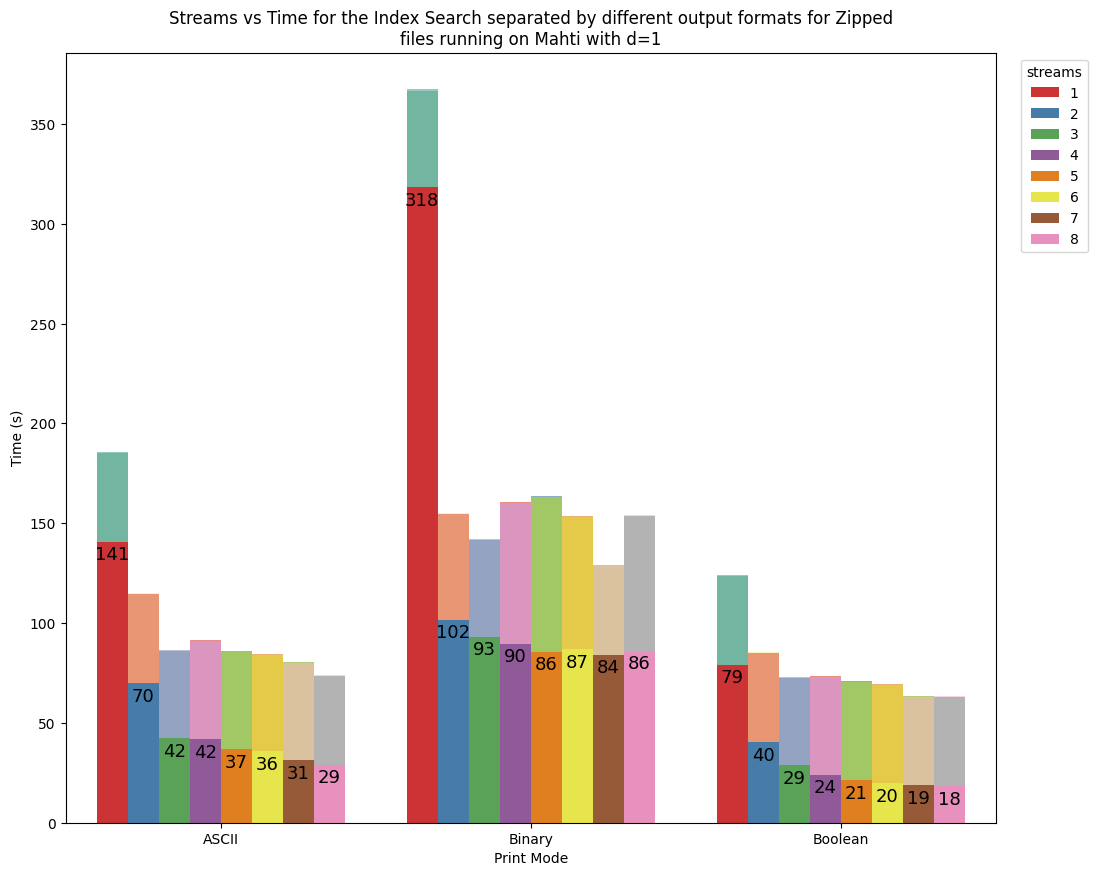
\includegraphics[width=0.7\textwidth]{images/MahtiIndexZippedD1.png}
  \caption{Timings for the Index Search with zipped inputs and $d=1$ on Mahti.}\label{fig:MahtiIndexZippedD1}
\end{figure}

\begin{figure}[t]
  \centering
  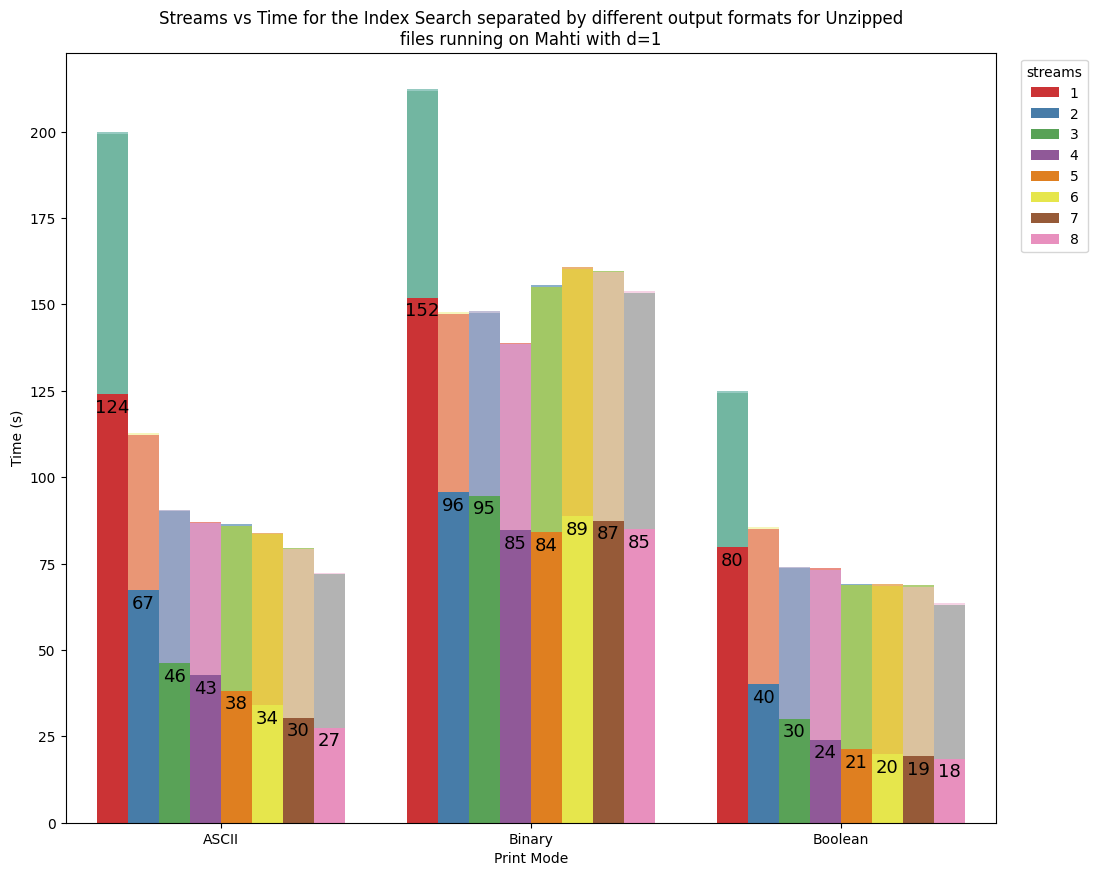
\includegraphics[width=0.7\textwidth]{images/MahtiIndexUnzippedD1.png}
  \caption{Timings for the Index Search with unzipped inputs and $d=1$ on Mahti.}\label{fig:MahtiIndexUnzippedD1}
\end{figure}

\begin{figure}[t]
  \centering
  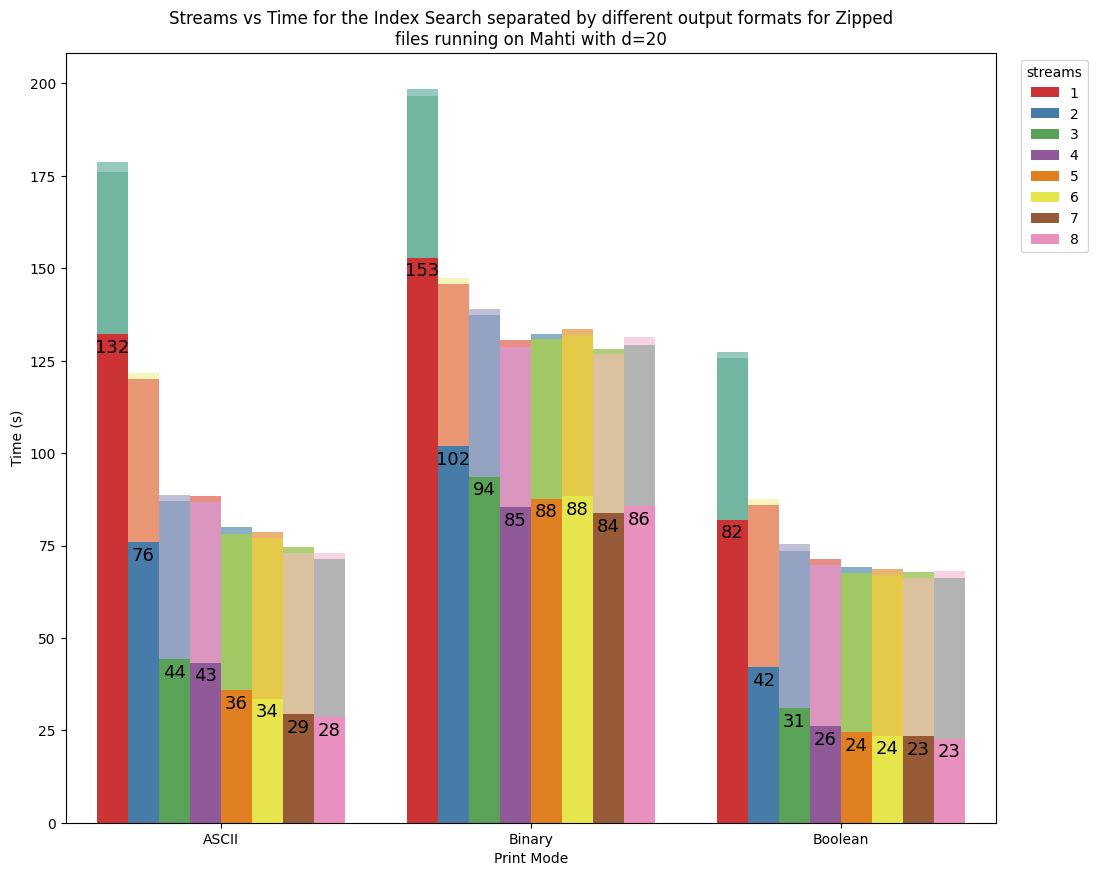
\includegraphics[width=0.7\textwidth]{images/MahtiIndexZippedD20.png}
  \caption{Timings for the Index Search with zipped inputs and $d=20$ on Mahti.}\label{fig:MahtiIndexZippedD20}
\end{figure}

\begin{figure}[t]
  \centering
  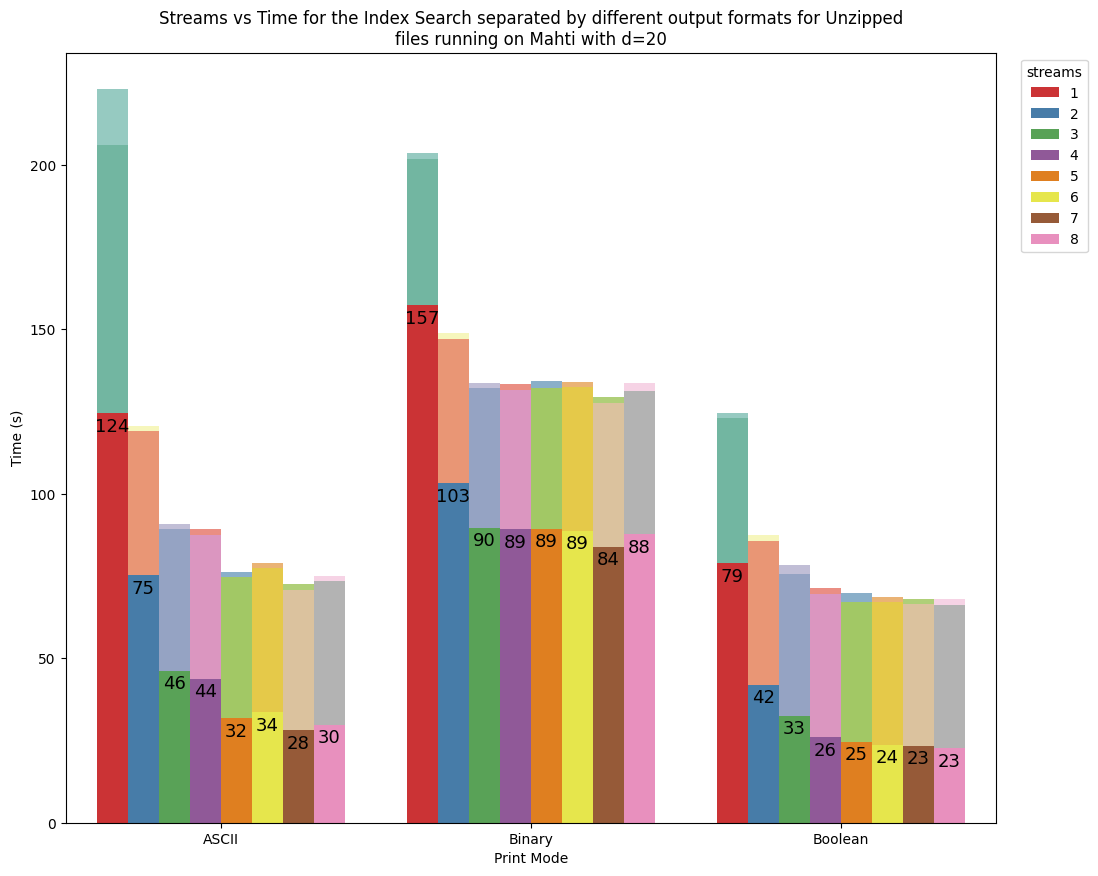
\includegraphics[width=0.7\textwidth]{images/MahtiIndexUnzippedD20.png}
  \caption{Timings for the Index Search with unzipped inputs and $d=20$ on Mahti.}\label{fig:MahtiIndexUnzippedD20}
\end{figure}

The main result format which will be focused on from the Index Search will be the ASCII format.
The reason for this is that it is the format that produces the least output, while being the fastest format which is also suitable for pseudoalignment.
It can be seen that when a single stream is considered, the I/O causes a large bottleneck since neither GPU I/O nor disk I/O is being parallelised.
The choice of the checkpoint parameter $d$ does not make much of a difference, even though the GPU kernel does more work.
This indicates that the kernel for searching is not the bottleneck.
There is also no significant difference between using the zipped or unzipped input format.

Stemming from these results, more focus will now be given to the results with the unzipped input with $d=20$.
The reasons are that the unzipped input was also given to Themisto, and the index with $d=20$ is also more scalable since the color set uses less space.
When using eight streams, the time taken to perform the search is 30 seconds, which is a throughput of 1.675 GB/s.
Figure~\ref{fig:MahtiIndexUnzippedD20S8ASCII} shows the timeline and a statistics table for this run.
One can see that most components run in parallel to each other, and even the same component type in different streams tend to run in parallel.
If the attention is then turned to the table in the same figure, whose description for each of its components can be found in Appendix~\ref{app:IndexTableDescriptions}, one may then infer that the most expensive phases are the parser which reads the files to disk, and the printer which outputs the results to disk.
This is seen in the \textit{max\_stream\_time} column, since the \textit{total\_time} column comprises the time taken by all the streams, even when they were working in parallel.
Focusing then on Figure~\ref{fig:MahtiIndexUnzippedD20S1ASCII}, which is the figure with a single stream, the reader may see the same trend, further enforcing earlier claims.

\begin{figure}[t]
  \centering
  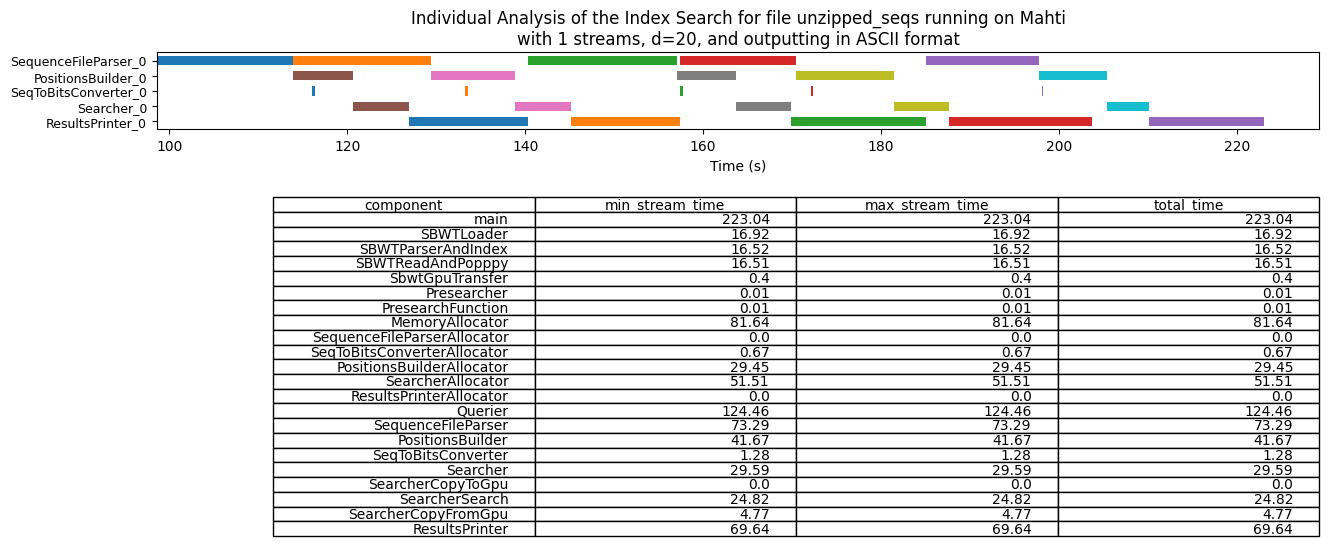
\includegraphics[width=\textwidth]{images/MahtiIndexUnzippedD20S1ASCII.png}
  \caption{Timeline for the Index Search running on Mahti with unzipped sequences as inputs, producing the ASCII format with $d=20$ and 1 streams, excluding loading and memory allocation.}\label{fig:MahtiIndexUnzippedD20S1ASCII}
\end{figure}

\begin{figure}[t]
  \centering
  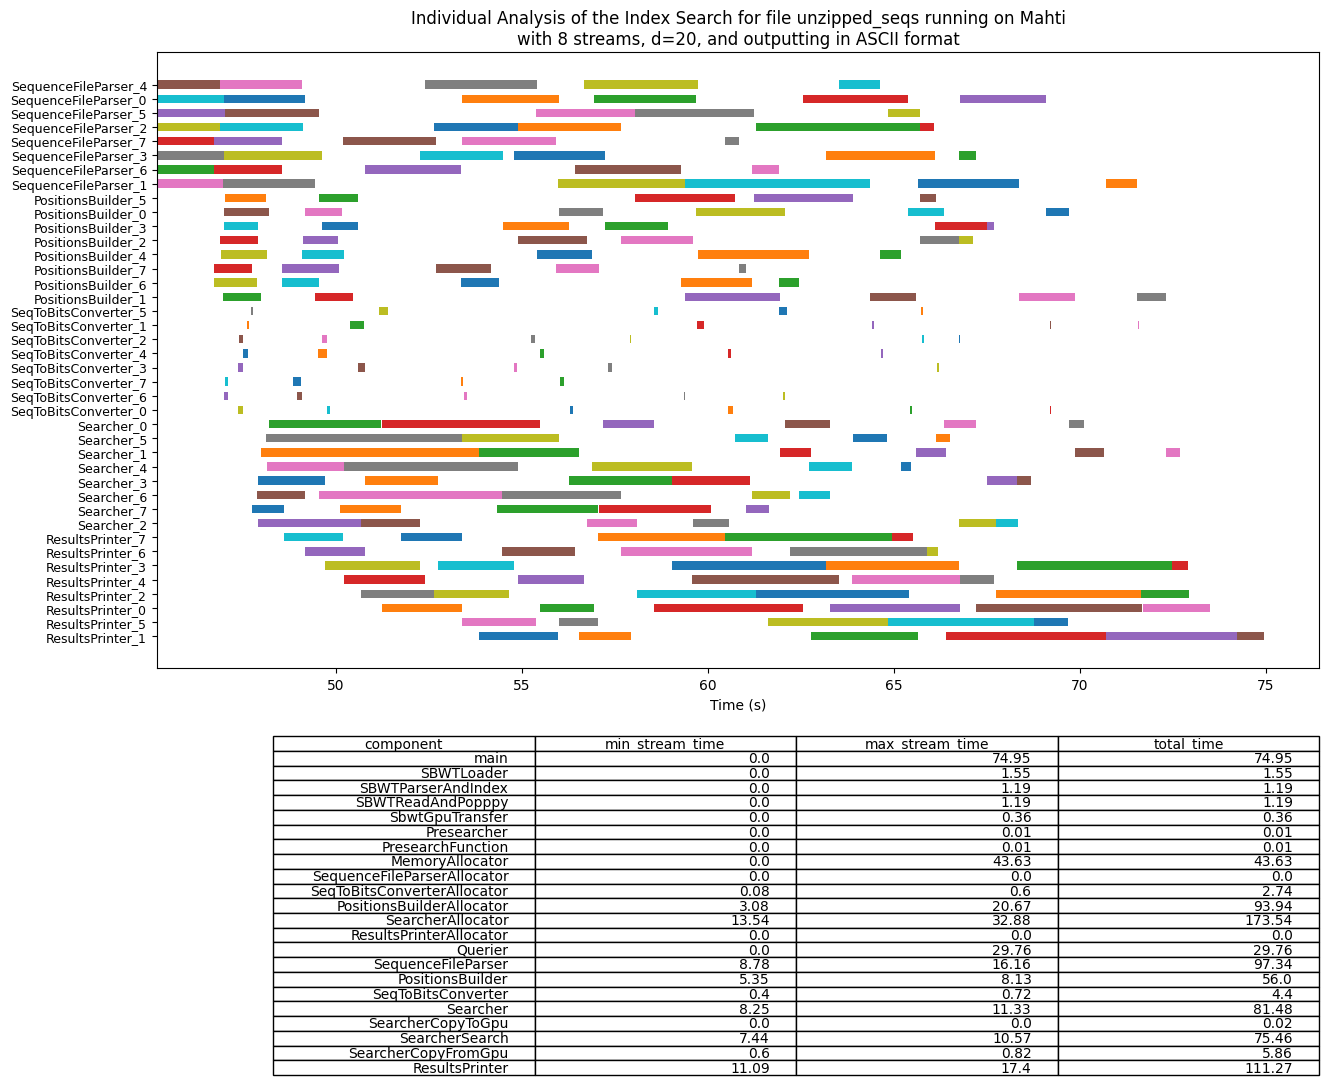
\includegraphics[width=\textwidth]{images/MahtiIndexUnzippedD20S8ASCII.png}
  \caption{Timeline for the Index Search running on Mahti with unzipped sequences as inputs, producing the ASCII format with $d=20$ and 8 streams, excluding loading and memory allocation.}\label{fig:MahtiIndexUnzippedD20S8ASCII}
\end{figure}

\subsection{LUMI}

On LUMI the story is a little different.
Note that, from now on, only the results with $d=20$ will be shown, as the results with $d=1$ are not scalable to larger indexes and the throughput is not significantly different.
In that same vein, only the unzipped sequences will be shown since these are the files whose size on which throughput is calculated on.
The first noticeable difference in Figure~\ref{fig:LumiIndexUnzippedD20} is that LUMI takes longer to process the results.
An anomaly consistently shows up for the index search with the boolean format, where the single stream outperforms multi-stream processing.
This seems to be coming from the kernel search function, which takes a much longer time as the number of streams increases.
However, the CPU processing then benefits from this as there is also multithreading there.
This may be observed from Figures~\ref{fig:LumiIndexUnzippedD20S1Boolean} and~\ref{fig:LumiIndexUnzippedD20S8Boolean}, which show the results with one and eight streams respectively.

\begin{figure}[t]
  \centering
  \includegraphics[width=0.7\textwidth]{images/LumiIndexUnzippedD20.png}
  \caption{Timings for the Index Search with unzipped inputs and d=20 on LUMI.}\label{fig:LumiIndexUnzippedD20}
\end{figure}


The results obtained for the ASCII format show a similar trend, as seen in Figures\ref{fig:LumiIndexUnzippedD20S1ASCII}  and~\ref{fig:LumiIndexUnzippedD20S8ASCII}.
As the number of streams increases, the longer the GPU kernels take.
However, since the CPU and I/O multithreading benefit from using multiple streams,
The reason for this difference, where the GPU kernel time is proportional to the streams is generally unknown, and will need to be further explored in future work beyond this thesis.
However, some possible reasons may be due to the AMD device doing fewer optimisations to the GPU kernel, or it is more susceptible to thread divergence, or the AMD device handles GPU random memory accesses worse than NVIDIA.
On LUMI, the average time taken for this index search when the number of streams is high enough, is around 120 seconds, which indicates a throughput of 418.9 MB/s.

\begin{figure}[t]
  \centering
  \includegraphics[width=\textwidth]{images/LumiIndexUnzippedD20S1Boolean.png}
  \caption{Timeline for the Index Search running on LUMI with unzipped sequences as inputs, producing the boolean format with $d=20$ and 1 streams, excluding loading and memory allocation.}\label{fig:LumiIndexUnzippedD20S1Boolean}
\end{figure}

\begin{figure}[t]
  \centering
  \includegraphics[width=\textwidth]{images/LumiIndexUnzippedD20S8Boolean.png}
  \caption{Timeline for the Index Search running on LUMI with unzipped sequences as inputs, producing the boolean format with $d=20$ and 8 streams, excluding loading and memory allocation.}\label{fig:LumiIndexUnzippedD20S8Boolean}
\end{figure}

\begin{figure}[t]
  \centering
  \includegraphics[width=\textwidth]{images/LumiIndexUnzippedD20S1ASCII.png}
  \caption{Timeline for the Index Search running on LUMI with unzipped sequences as inputs, producing the ASCII format with $d=20$ and 1 streams, excluding loading and memory allocation.}\label{fig:LumiIndexUnzippedD20S1ASCII}
\end{figure}

\begin{figure}[t]
  \centering
  \includegraphics[width=\textwidth]{images/LumiIndexUnzippedD20S8ASCII.png}
  \caption{Timeline for the Index Search running on LUMI with unzipped sequences as inputs, producing the ASCII format with $d=20$ and 8 streams, excluding loading and memory allocation.}\label{fig:LumiIndexUnzippedD20S8ASCII}
\end{figure}

\section{Color Search}

The next set of results arise from the second phase of pseudoalignment, which is the Color Search.
For this phase, the user may choose to read from the ASCII or the binary output of the first phase.
The results for $d=1$ and $d=20$ will be approximately the same, since the same work needs to be done in this phase, hence focus will be shifted towards $d=20$.
The size of the resulting ASCII and binary formats are 110 GB and 180 GB respectively.
Regarding the CSV format, this leads to files that are too large, so no results will be given for this format.
This format is only recommended for extremely dense outputs.

\subsection{Mahti}

When looking at Figure~\ref{fig:MahtiColorASCIID20}, one can, first of all, see a large difference between one stream and two.
The graph shows a decaying exponential decrease in the time taken, as more streams are added, going down to less than 70 seconds at seven and eight streams when it comes to the ASCII output format, when not considering startup.
Based on the result from the indexes, which was 49 GB, this means that this part has a throughput of 49 GB / 70s = 700 MB/s.
Meanwhile, from the FASTQ files, the total throughput of our method is $50.265$ / (30 + 70)s $\approx$ 500 MB/s, which is 17.5x faster than the best result from Themisto on the same 32 cores, or 10x times faster than when Themisto is run on 64 cores on LUMI.
The ASCII format is again much faster than the boolean format as it needs to perform less disk I/O.
To gain insight on the performance bottlenecks in this case, Figure~\ref{fig:MahtiColorASCIID20S8ASCII} shows the run with the ASCII output with eight streams.
The I/O, especially output, is the biggest bottleneck.
Copying the results from GPU to CPU memory also takes quite a long time, while the rest of the components are almost insignificant in comparison to the mentioned parts.

\begin{figure}[t]
  \centering
  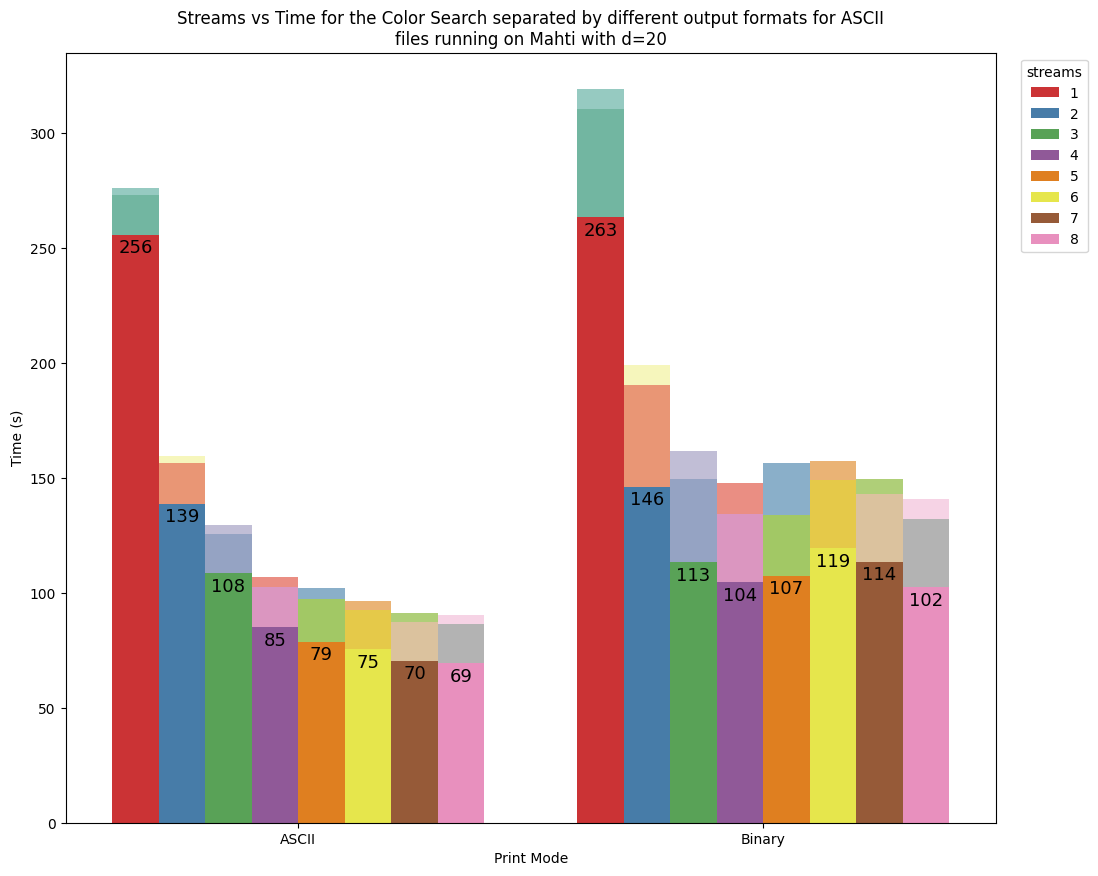
\includegraphics[width=0.7\textwidth]{images/MahtiColorASCIID20.png}
  \caption{Timing results for the Color Search, reading from the ASCII indexes, with $d=20$ running on Mahti}\label{fig:MahtiColorASCIID20}
\end{figure}

\begin{figure}[t]
  \centering
  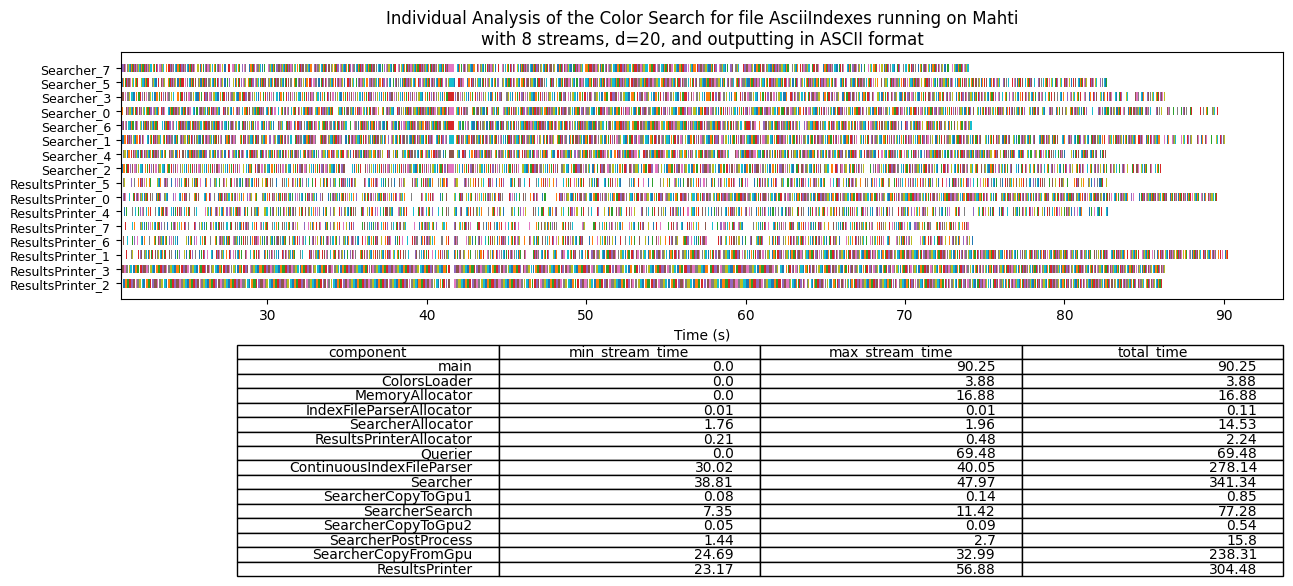
\includegraphics[width=\textwidth]{images/MahtiColorASCIID20S8ASCII.png}
  \caption{Timeline for the Color Search running on Mahti with ASCII indexes as inputs, producing the ASCII format with $d=20$ and 8 streams, excluding loading and memory allocation.}\label{fig:MahtiColorASCIID20S8ASCII}
\end{figure}

\subsection{LUMI}

Similar to the Index Search, the Color Search on LUMI is faster on the CPU side of things, but significantly slower on the GPU.
Figure~\ref{fig:LumiColorASCIID20} shows the overall results of the Color Search when reading from the ASCII indexes.
This time, there is less difference between using a single stream or multiple streams.
The results are also less consistent, with a remaining uncertainty in why this is the case.
With Figure~\ref{fig:LumiColorASCIID20S8ASCII}, which shows the run with eight streams, one may see that most time is taken with the searching part of this phase.
Everything else is faster than when run on Mahti with a moderate margin.

\begin{figure}[t]
  \centering
  \includegraphics[width=0.7\textwidth]{images/LumiColorASCIID20.png}
  \caption{Timing results for the Color Search, reading from the ASCII indexes, with $d=20$ running on LUMI}\label{fig:LumiColorASCIID20}
\end{figure}

\begin{figure}[t]
  \centering
  \includegraphics[width=\textwidth]{images/LumiColorASCIID20S8ASCII.png}
  \caption{Timeline for the Color Search running on LUMI with ASCII indexes as inputs, producing the ASCII format with $d=20$ and 8 streams, excluding loading and memory allocation.}\label{fig:LumiColorASCIID20S8ASCII}
\end{figure}

With an average time taken of 450s, when considering that the indexes read are 49 GB, this phase has a throughput of 109 MB/s.
If the entire pipeline is considered, with the FASTQ inputs of $50.265$ GB, then the end-to-end throughput is $50.265$ / (120s + 450s) $\approx$ 88MB/s, which is 70\% faster than Themisto.
Thus, even though the GPU kernel is much slower than on Mahti, the gains are still substantial enough to consider using, given a large enough dataset.
